
\begin{enumerate}[\Large\bfseries 1.]

%--------------------1.
\item 
\begin{enumerate}[\bfseries a)]
    
    %----------a)
    \item \textbf{Análisis del problema.}\\

    Sea $V = \pi \cdot r^2 \cdot h$ entonces 
	\begin{center}
	    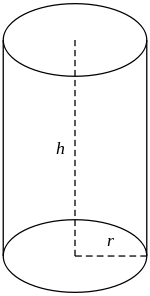
\includegraphics[scale=0.5]{imagenes/tarea2/cilindro.png} \\
	\end{center}

    por lo tanto si $r=2$, $h=3$ implica que $$v=\pi\cdot 2**2\cdot 3 = 12\pi.$$\\

    %----------b)
    \item \textbf{Diagrama de flujo.}\\
	\begin{center}
	    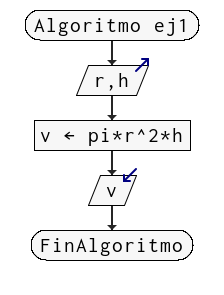
\includegraphics[scale=.9]{imagenes/tarea2/ej1df.png}
	\end{center}

    %----------c)
    \item \textbf{Prueba de escritorio.}\\
	\begin{center}
	    \begin{tabular}{c|c|c}
		r&h&v\\
		\hline
		2&3&12$\pi$\\
	    \end{tabular}
	\end{center}
	\vspace{1cm}
    
    %----------d)
    \item \textbf{Código fuente.}\\ 
	
	\lstinputlisting[language=Python]{python/tarea2/ej1.py}
	\vspace{1cm}
    
    %----------e)
    \item \textbf{Prueba de la ejecución del programa}.\\
	\begin{center}
	    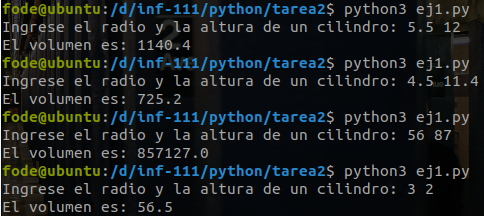
\includegraphics[scale=.7]{imagenes/tarea2/ej1.png}
	\end{center}

\end{enumerate}

\newpage

%-------------------2.
\item 
\begin{enumerate}[\bfseries a)]
    
    %----------a)
    \item \textbf{Análisis del problema.}\\\\
    Sea 
	\begin{center}
	    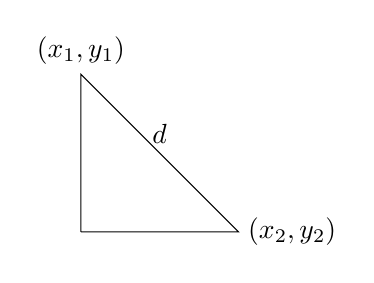
\begin{tikzpicture}
		\draw(0,0)--(0,2)node[above]{$(x_1,y_1)$}--(2,0)node[right]{$(x_2,y_2)$}--(0,0);
		\draw(1,1)node[above]{$d$};
	    \end{tikzpicture}
	\end{center}
	entonces $$\left[(x_2-x_1)^2+(y_2-y_1)^2\right]^{1/2}$$
	luego si tenemos $x_1=1$, $x_2=2$, $y_1=3$ y $y_2=4$ se obtiene, $$d=\left[(2-1)^2+(4-3)^2\right]^{1/2} = 1.$$\\	

    %----------b)
    \item \textbf{Diagrama de flujo.}\\
	\begin{center}
	    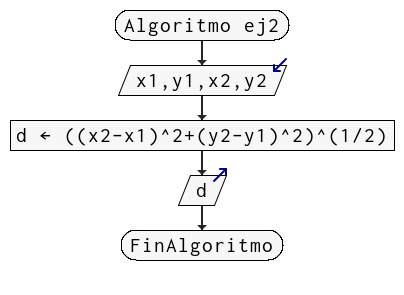
\includegraphics[scale=.9]{imagenes/tarea2/ej2df.png}
	\end{center}

    %----------c)
    \item \textbf{Prueba de escritorio.}\\\\
	\begin{center}
	    \begin{tabular}{c|c|c|c|c}
		x1&y1&x2&y2&d\\	
		\hline
		1&3&2&4&$\sqrt{2}$\\
	    \end{tabular}
	\end{center}
	\vspace{2cm}
    
    %----------d)
    \item \textbf{Código fuente.}\\ 
	
	\lstinputlisting[language=Python]{python/tarea2/ej2.py}
	\vspace{1cm}
    
    %----------e)
    \item \textbf{Prueba de la ejecución del programa}.\\
	\begin{center}
	    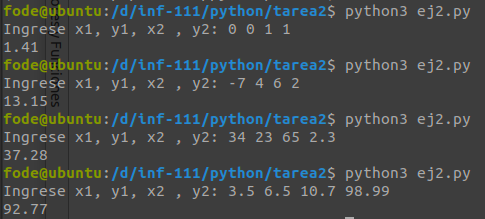
\includegraphics[scale=.7]{imagenes/tarea2/ej2.png}
	\end{center}

\end{enumerate}

\newpage


%-------------------3.
\item 
\begin{enumerate}[\bfseries a)]
    
    %----------a)
    \item \textbf{Análisis del problema.}\\\\
    Supongamos que se tiene un precio $$p=4$$ donde se aplica a un descuento del $10\%$. Para ello se tiene $$d=p\cdot 0.1 \; \Longrightarrow \; d = 4\cdot 0.1 = 0.4$$
    Así el precio a pagar será $$tp = p-d \; \Longrightarrow \; tp = 4-0.4 = 3.6$$\\

    %----------b)
    \item \textbf{Diagrama de flujo.}\\
	\begin{center}
	    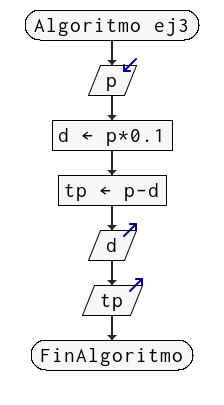
\includegraphics[scale=.9]{imagenes/tarea2/ej3df.png}
	\end{center}
	\vspace{1cm}

    %----------c)
    \item \textbf{Prueba de escritorio.}\\\\
	\begin{center}
	    \begin{tabular}{c|c|c}
		p&d&tp\\
		\hline
		4&0.4&3.6\\
	    \end{tabular}
	\end{center}
	\vspace{2cm}
    
    %----------d)
    \item \textbf{Código fuente.}\\ 
	
	\lstinputlisting[language=Python]{python/tarea2/ej3.py}
	\vspace{1cm}
    
    %----------e)
    \item \textbf{Prueba de la ejecución del programa}.\\
	\begin{center}
	    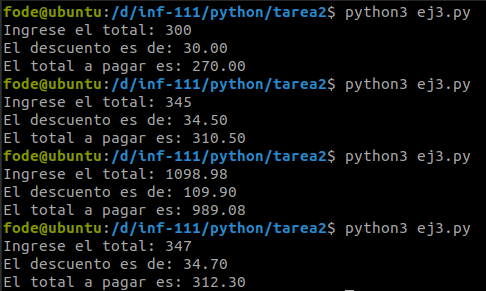
\includegraphics[scale=.7]{imagenes/tarea2/ej3.png}
	\end{center}

\end{enumerate}

\newpage


%-------------------4.
\item 
\begin{enumerate}[\bfseries a)]
    
    %----------a)
    \item \textbf{Análisis del problema.}\\\\
    Sea $hombres = x$ y $mujeres = z$, entonces el porcentaje $\%$ viene dado por 
	$$h = \dfrac{x}{x+z}\cdot 100$$
	$$m = \dfrac{y}{x+z}\cdot 100$$
	si $x=10$ y $z=20$ se tiene,
	$$h = \dfrac{10}{10+20}\cdot 100 = 33.33\%$$
	$$h = \dfrac{20}{10+20}\cdot 100 = 66.66\%$$\\

    %----------b)
    \item \textbf{Diagrama de flujo.}\\
	\begin{center}
	    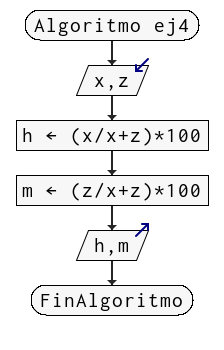
\includegraphics[scale=.9]{imagenes/tarea2/ej4df.png}
	\end{center}
	\vspace{1cm}

    %----------c)
    \item \textbf{Prueba de escritorio.}\\\\
	\begin{center}
	    \begin{tabular}{c|c|c|c}
		x&y&h&m\\
		\hline
		6&4&60&40\\
	    \end{tabular}
	\end{center}
	\vspace{1cm}
    
    %----------d)
    \item \textbf{Código fuente.}\\ 
	
	\lstinputlisting[language=Python]{python/tarea2/ej4.py}
	\vspace{1cm}
    
    %----------e)
    \item \textbf{Prueba de la ejecución del programa}.\\
	\begin{center}
	    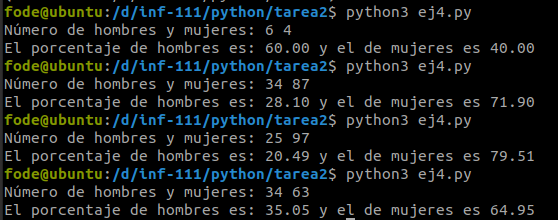
\includegraphics[scale=.7]{imagenes/tarea2/ej4.png}
	\end{center}

\end{enumerate}

\newpage


%-------------------5.
\item 
\begin{enumerate}[\bfseries a)]
    
    %----------a)
    \item \textbf{Análisis del problema.}\\\\
	Sea $x$ la distancia entonces los kilómetros que se recorrerá por litro estarán dados por $$kl = \dfrac{x}{y}$$
	donde $y$ son los kilómetros por litro. Luego el costo estará dado por $$c = kl\cdot p,$$ para $p$ iguala precio.\\\\


    %----------b)
    \item \textbf{Diagrama de flujo.}\\
	\begin{center}
	    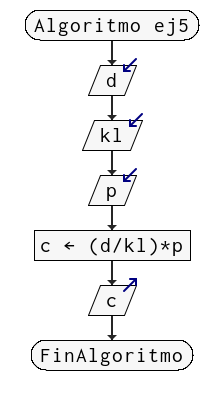
\includegraphics[scale=.9]{imagenes/tarea2/ej5df.png}
	\end{center}
	\vspace{.5cm}

    %----------c)
    \item \textbf{Prueba de escritorio.}\\\\
	\begin{center}
	    \begin{tabular}{c|c|c|c}
		d&kl&p&c\\
		\hline
		80&8&3.2&32\\
	    \end{tabular}
	\end{center}
	\vspace{1cm}
    
    %----------d)
    \item \textbf{Código fuente.}\\ 
	
	\lstinputlisting[language=Python]{python/tarea2/ej5.py}
	\vspace{1cm}
    
    %----------e)
    \item \textbf{Prueba de la ejecución del programa}.\\
	\begin{center}
	    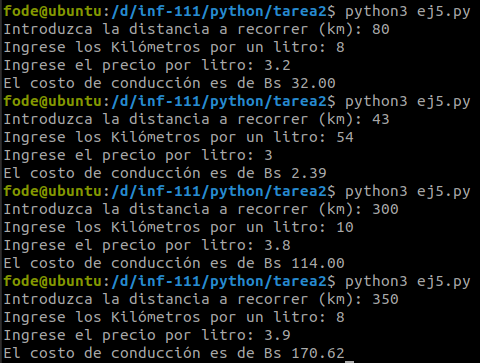
\includegraphics[scale=.7]{imagenes/tarea2/ej5.png}
	\end{center}

\end{enumerate}

\newpage


%-------------------6.
\item 
\begin{enumerate}[\bfseries a)]
    
    %----------a)
    \item \textbf{Análisis del problema.}\\\\
	Sea $min$ los minutos dados, entonces empezamos convirtiendo los minutos a años y días de la siguiente manera $$conv = min\cdot \dfrac{1}{60}\cdot \dfrac{1}{24}\cdot\dfrac{1}{365}$$
	de donde los años vienen dados por por entero del resultado correspondiente $$años = int(conv)$$
	luego, los decimales los convertimos en días con la siguiente formula:
	$$p_e =abs(conv) - abs(int(conv))$$
	para luego $$dias = p_d\cdot 365$$\\


    %----------b)
    \item \textbf{Diagrama de flujo.}\\
	\begin{center}
	    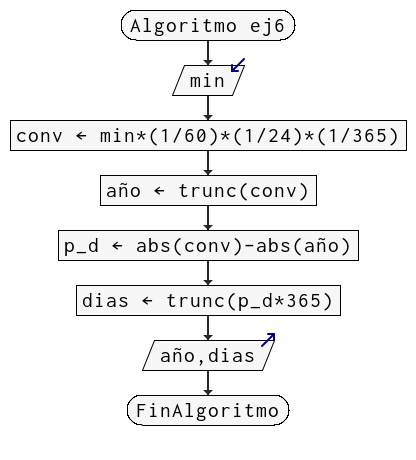
\includegraphics[scale=.7]{imagenes/tarea2/ej6df.png}
	\end{center}
	\vspace{1cm}

    %----------c)
    \item \textbf{Prueba de escritorio.}\\\\
	\begin{center}
	    \begin{tabular}{c|c|c|c|c}
		min&conv&año&p\_d&dias\\
		\hline
		1000000000&1902.58&1902&0.58&214\\
	    \end{tabular}
	\end{center}
	\vspace{1cm}
    
    %----------d)
    \item \textbf{Código fuente.}\\ 
	
	\lstinputlisting[language=Python]{python/tarea2/ej6.py}
	\vspace{1cm}
    
    %----------e)
    \item \textbf{Prueba de la ejecución del programa}.\\
	\begin{center}
	    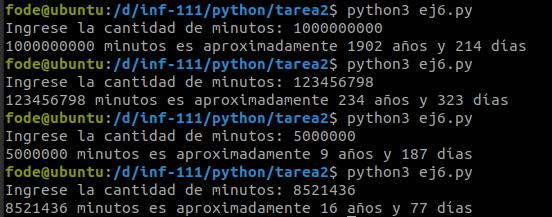
\includegraphics[scale=.7]{imagenes/tarea2/ej6.png}
	\end{center}

\end{enumerate}

\newpage


%-------------------7.
\item 
\begin{enumerate}[\bfseries a)]
    
    %----------a)
    \item \textbf{Análisis del problema.}\\\\
	Sea $mt$ el monto total y $p$ el porcentaje de propina entonces el monto de la propina viene dado por $$mp = m\cdot \dfrac{p}{100}$$
	de donde el total a pagar será $$tp = mt + mp$$\\

    %----------b)
    \item \textbf{Diagrama de flujo.}\\
	\begin{center}
	    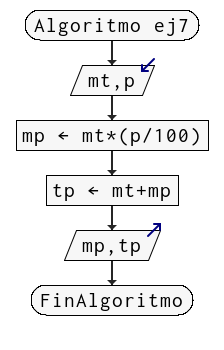
\includegraphics[scale=.9]{imagenes/tarea2/ej7df.png}
	\end{center}
	\vspace{1cm}

    %----------c)
    \item \textbf{Prueba de escritorio.}\\\\
	\begin{center}
	    \begin{tabular}{c|c|c|c}
		mt&p&mp&tp\\
		\hline
		10&15&1.5&11.5\\
	    \end{tabular}
	\end{center}
	\vspace{3cm}
    
    %----------d)
    \item \textbf{Código fuente.}\\ 
	
	\lstinputlisting[language=Python]{python/tarea2/ej7.py}
	\vspace{1cm}
    
    %----------e)
    \item \textbf{Prueba de la ejecución del programa}.\\
	\begin{center}
	    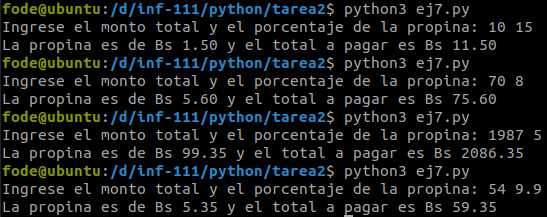
\includegraphics[scale=.7]{imagenes/tarea2/ej7.png}
	\end{center}

\end{enumerate}

\newpage


%-------------------8.
\item 
\begin{enumerate}[\bfseries a)]
    
    %----------a)
    \item \textbf{Análisis del problema.}\\\\
	Primero debemos extraer el número introducido, dígito por dígito, para posteriormente sumarlos. Para tal efecto tomamos el módulo (resto de la división) de un número cualquiera $n$ de la siguiente manera:
	$$n \% 10$$ por ejemplo si $n=932$ entonces, $932\%10 = 2$ o $n=76$ entonces, $76\%10 = 6$. Así, si iteramos las veces que sea necesario nos dará la suma de todos los dígitos de $n$. Cabe recordar que es necesario actualizar el número $n$ para extraer el segundo dígito como sigue:
	$$n//10$$
	Por ejemplo, si tomamos $n=932$ entonces $932//10=93$ donde se ve claramente que es la división entera de la división.
	En este caso no importa si extraemos el dígito por la derecha o por la izquierda. Todo este procedimiento se debe realizar hasta que la división entera sea igual a cero, para ello recurrimos a un iterador while.\\\\

    %----------b)
    \item \textbf{Diagrama de flujo.}\\
	\begin{center}
	    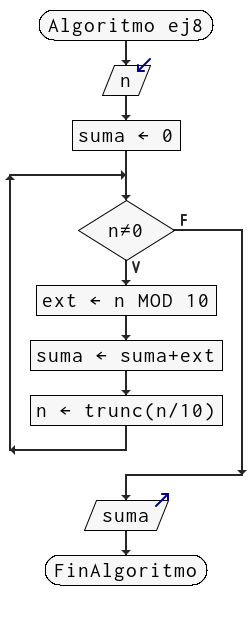
\includegraphics[scale=.65]{imagenes/tarea2/ej8pf.png}
	\end{center}
	\vspace{1cm}

    %----------c)
    \item \textbf{Prueba de escritorio.}\\\\
	\begin{center}
	    \begin{tabular}{c|c|c|c}
		n&suma&ext&print\\
		\hline
		$\cancel{932}$&$\cancel{0}$&$\cancel{2}$&14\\
		$\cancel{93}$&$\cancel{2}$&$\cancel{3}$&\\
		$\cancel{9}$&$\cancel{5}$&$9$&\\
		$0$&$14$&&\\
	    \end{tabular}
	\end{center}
	\vspace{1cm}
    
    %----------d)
    \item \textbf{Código fuente.}\\ 
	
	\lstinputlisting[language=Python]{python/tarea2/ej8.py}
	\vspace{1cm}
    
    %----------e)
    \item \textbf{Prueba de la ejecución del programa}.\\
	\begin{center}
	    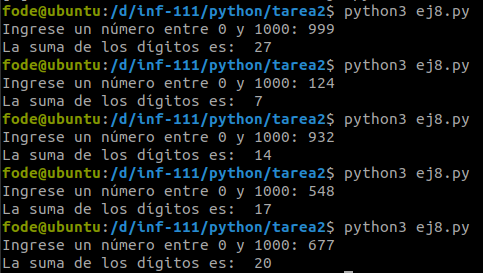
\includegraphics[scale=.7]{imagenes/tarea2/ej8.png}
	\end{center}

\end{enumerate}

\newpage


%-------------------9.
\item 
\begin{enumerate}[\bfseries a)]
    
    %----------a)
    \item \textbf{Análisis del problema.}\\\\
	Primeramente convertimos un año en segundos:
	$$conv=365*24*60*60$$
	con este hecho podemos averiguar cuantas personas nacen, cuantas mueren y cuantas emigran en un año, simplemente dividiendo los datos brindados al resultado de $conv$, es decir:
	$$nacen = \dfrac{conv}{7}, \qquad mueren = \dfrac{conv}{13},\qquad emigran = \dfrac{conv}{45}$$
	Por otro lado la población que se estimará estará dada por:
	$$pob = nacen - mueren + emigran$$
	así nos queda: $$pob = conv\left(\dfrac{1}{7}-\dfrac{1}{13}+\dfrac{1}{45}\right)$$
	de donde al multiplicar por los años que se introducirá y sumado a la población actual nos queda:
	$$pob\_total = 312032486 + (\mbox{año}*pob)$$\\

    %----------b)
    \item \textbf{Diagrama de flujo.}\\
	\begin{center}
	    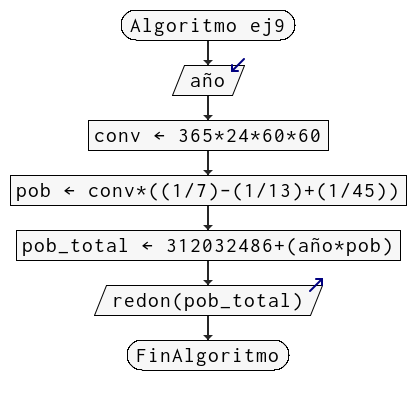
\includegraphics[scale=.9]{imagenes/tarea2/ej9df.png}
	\end{center}
	\vspace{1cm}

    %----------c)
    \item \textbf{Prueba de escritorio.}\\\\
	\begin{center}
	    \begin{tabular}{c|c|c|c}
		año&conv&pob&pob$\_$total\\
		\hline
		5&31536000&2780096.7033&325932970\\
	    \end{tabular}
	\end{center}
	\vspace{1cm}
    
    %----------d)
    \item \textbf{Código fuente.}\\ 
	
	\lstinputlisting[language=Python]{python/tarea2/ej9.py}
	\vspace{1cm}
    
    %----------e)
    \item \textbf{Prueba de la ejecución del programa}.\\
	\begin{center}
	    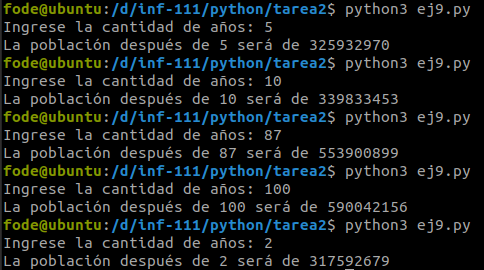
\includegraphics[scale=.7]{imagenes/tarea2/ej9.png}
	\end{center}

\end{enumerate}

\newpage


%-------------------10.
\item 
\begin{enumerate}[\bfseries a)]
    
    %----------a)
    \item \textbf{Análisis del problema.}\\\\
	Sea $" total "$ el total a pagar y $"pago"$ el pago que se realiza, entonces, la diferencia estará dada por $"cambio"$ que es el cambio que recibirá el cliente.\\
	Para poder encontrar  $"cambio"$ fraccionado en monedas de 5, 2, 1, 0.50, 0.20 y 0.10 dado en $Bs.$\\ Dividiremos $"cambio"$ por cada fracción en monedas de manera descendente, siempre tomando por separando la parte entera de los decimales, para luego tomar la parte decimal y convertirlo al resto correspondiente,  es decir:\\\\
	Supongamos que $"cambio"$ es igual a $18.8$ de donde
	\begin{center} $[cinco] = \left[\dfrac{18.8}{5}\right] = [3.76] = 3$\end{center}  
	    en esta parte se tomo la parte entera $"$piso$"$ para que $cinco=3$. Procedemos luego a encontrar el resto de la división como sigue, $$cambio=5\cdot\left(\dfrac{18.8}{5}-[cinco] \right) = 3.8$$
	    Para hallar correctamente el resto, el cual será el nuevo $"cambio"$, es necesario multiplicar la diferencia por $5$ ya que anteriormente se dividio por el mismo resultado.\\\\
	    Ahora que se actualizo $"cambio"$ tenemos que este vale 3.8, así,
	    $$[dos] = \left[\dfrac{3.8}{2}\right] = [1.6] = 1 \qquad y \qquad cambio = 2\cdot\left(\dfrac{3.8}{2} - [dos]\right) = 1.8$$\\
	    Lo mismo  para 1, con $cambio =$ 1.8,
	    $$\left[uno\right] = \left[\dfrac{1.8}{1}\right] = \left[1.8\right] = 1 \qquad y \qquad cambio = 1 \cdot \left(\dfrac{1.8}{1} - [uno]\right) = 0.8$$\\
	    para 0.5, con $"cambio" =$ 0.8,

	    $$\left[cincuenta\right] = \left[\dfrac{0.8}{0.5}\right] = \left[1.6\right] = 1 \qquad y \qquad cambio = 0.5 \cdot \left(\dfrac{0.8}{0.5} - [cincuenta]\right) = 0.3$$\\
	    
	    para 0.2, con $cambio = $ 0.3,

	    $$\left[veinte\right] = \left[\dfrac{0.3}{0.2}\right] = \left[1.5\right] = 1 \qquad y \qquad cambio = 0.2 \cdot \left(\dfrac{0.3}{0.2} - [veinte]\right) = 0.1$$\\
    
	    y para 0.1, con $cambio = $ 0.1,
	    
	    $$\left[diez\right] = \left[\dfrac{0.1}{0.1}\right] = \left[1\right] = 1 \qquad y \qquad cambio = 0.1 \cdot \left(\dfrac{0.1}{0.1} - [diez]\right) = 1$$\\\\
	    \vspace{2cm}


    %----------b)
    \item \textbf{Diagrama de flujo.}\\
	\begin{center}
	    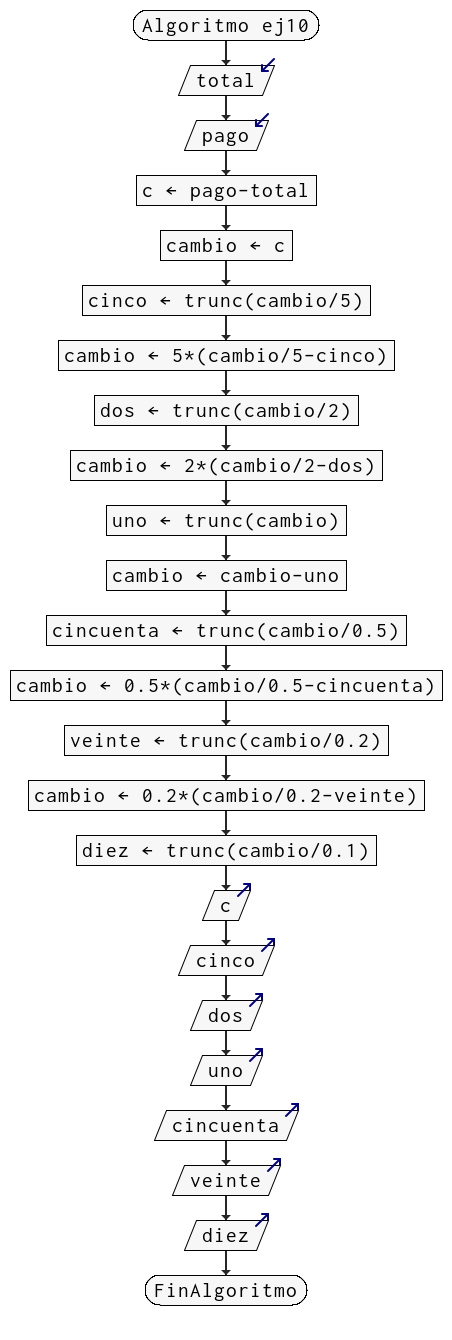
\includegraphics[scale=.45]{imagenes/tarea2/ej10df.png}
	\end{center}
	\vspace{1cm}

    %----------c)
    \item \textbf{Prueba de escritorio.}\\\\
	\begin{center}
	    \begin{tabular}{c|c|c|c|c|c|c|c|c}
		total&pago&cambio&cinco&dos&uno&cincuenta&veinte&diez\\
		\hline
		81.20&100&\cancel{18.8}&3&1&1&1&1&1\\
		&&\cancel{3.8}&&&&&&\\
		&&\cancel{1.8}&&&&&&\\
		&&\cancel{0.8}&&&&&&\\
		&&\cancel{0.3}&&&&&&\\
		&&0.1&&&&&&\\
	    \end{tabular}
	\end{center}
	\vspace{1cm}
    
    %----------d)
    \item \textbf{Código fuente.}\\ 
	
	\lstinputlisting[language=Python]{python/tarea2/ej10.py}
	\vspace{10cm}
    
    %----------e)
    \item \textbf{Prueba de la ejecución del programa}.\\
	\begin{center}
	    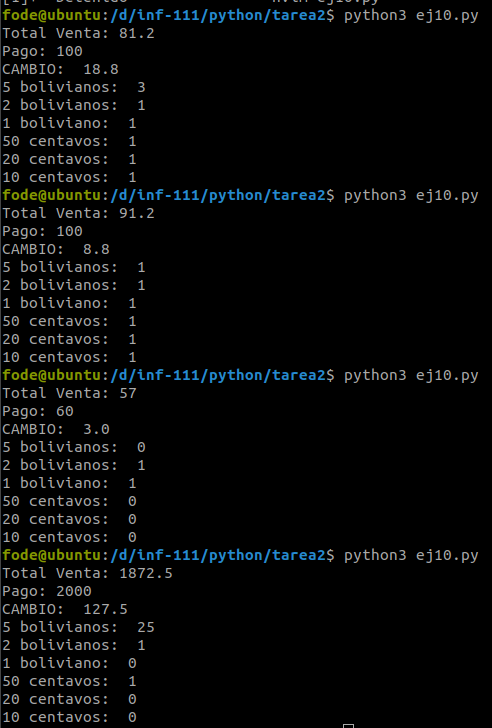
\includegraphics[scale=.7]{imagenes/tarea2/ej10.png}
	\end{center}

\end{enumerate}

\newpage
\end{enumerate}
